\documentclass[12pt,a4paper]{article}

% --- PACKAGES ---
\usepackage[margin=2.5cm]{geometry}
\usepackage{amsmath, amssymb, amsfonts}
\usepackage{graphicx}
\usepackage{booktabs}
\usepackage{xcolor}
\usepackage{listings}
\usepackage{enumitem}
\usepackage{fancyhdr}
\usepackage{hyperref}
\usepackage{tikz}
\usepackage{circuitikz}
\usetikzlibrary{calc, shadows}
\usepackage{float}
\usepackage{array}
\usepackage{multirow}

% --- THEME COLORS ---
\definecolor{SharifRed}{RGB}{185, 4, 0}
\definecolor{SharifDark}{RGB}{40, 45, 55}
\definecolor{SharifLight}{RGB}{174, 174, 174}
\definecolor{CalcGray}{RGB}{245, 245, 245}
\definecolor{CodeGreen}{RGB}{0, 150, 0}
\definecolor{CodeBlue}{RGB}{0, 0, 200}

% --- TCOLORBOX CONFIGURATION ---
\usepackage{tcolorbox}
\tcbuselibrary{skins, breakable}

\newtcolorbox{taskbox}[2][]{
    colback=SharifRed!5!white,
    colframe=SharifRed,
    coltitle=white,
    fonttitle=\bfseries\large,
    title={#2},
    arc=0mm,
    boxrule=1.5pt,
    enhanced jigsaw,
    breakable,
    drop shadow={opacity=0.25,shadow xshift=2pt,shadow yshift=-2pt},
    #1
}

\newtcolorbox{answerbox}[2][]{
    colback=white,
    colframe=SharifDark,
    coltitle=white,
    fonttitle=\bfseries\large,
    title={#2},
    arc=0mm,
    boxrule=1pt,
    enhanced jigsaw,
    breakable,
    lines before break=1,
    drop shadow={opacity=0.15,shadow xshift=1pt,shadow yshift=-1pt},
    #1
}

\newtcolorbox{calcbox}[2][]{
    colback=CalcGray,
    colframe=SharifLight,
    coltitle=black,
    fonttitle=\bfseries\large,
    title={#2},
    arc=0mm,
    boxrule=1.5pt,
    borderline={0.5pt}{0pt}{black!30!white,dashed},
    enhanced jigsaw,
    breakable,
    lines before break=1,
    drop shadow={opacity=0.15,shadow xshift=1pt,shadow yshift=-1pt},
    #1
}

% --- LISTINGS CONFIGURATION ---
\lstset{
    language=Python,
    backgroundcolor=\color{CalcGray},
    basicstyle=\ttfamily\scriptsize\selectfont,
    keywordstyle=\color{CodeBlue}\bfseries,
    commentstyle=\color{CodeGreen}\itshape,
    stringstyle=\color{SharifRed},
    showstringspaces=false,
    breaklines=true,
    numbers=left,
    numberstyle=\tiny\color{gray},
    frame=single,
    rulecolor=\color{SharifLight}
}

% --- PERSIAN LANGUAGE SUPPORT ---
\usepackage{xepersian}
\settextfont{XB Niloofar.ttf}
\setdigitfont{XB Niloofar.ttf}

% --- HEADER/FOOTER ---
\setlength{\headheight}{15pt}
\pagestyle{fancy}
\fancyhf{}
\rhead{\textcolor{SharifRed}{\textbf{گزارش پروژه الکترونیک ۲: فاز دوم}}}
\lhead{\textcolor{SharifRed}{\textbf{الکترونیک ۲}}}
\cfoot{\thepage}
\renewcommand{\headrulewidth}{1pt}
\renewcommand{\headrule}{\hbox to\headwidth{\color{SharifRed}\leaders\hrule height \headrulewidth\hfill}}

% --- HYPERLINKS SETUP ---
\hypersetup{
    colorlinks=true,
    linkcolor=SharifRed,
    urlcolor=cyan,
    pdftitle={Electronics 2 Project Phase 2 Report Template},
}

\begin{document}

% =============================================================================
% TITLE
% =============================================================================
\begin{center}
    \vspace*{0.5cm}
    {\huge \textbf{\textcolor{SharifDark}{گزارش طراحی و ارزیابی پروژه الکترونیک ۲\\(فاز دوم)}}} \\
    \vspace{0.5cm}
    \begin{tabular}{r l r l}
        \textbf{نام و نام خانوادگی:} & \underline{آریا فاتح کرداری} & \textbf{شماره دانشجویی:} & \underline{403110382} \\
    \end{tabular}
    \vspace{1cm}
    \hrule
\end{center}

\vspace{0.5cm}

% =============================================================================
% PROJECT REQUIREMENTS
% =============================================================================
\section{مشخصات مورد نیاز پروژه}

\begin{taskbox}{الزامات اصلی فاز دوم}
در این فاز باید مدار کامل‌شده‌ی تقویت‌کننده به‌گونه‌ای طراحی و ارزیابی شود که شامل ورودی تفاضلی، طبقات تقویت ولتاژ، مدارهای بایاس، طبقه‌ی خروجی توان، بار خروجی و فیدبک منفی سراسری باشد. مدار نهایی باید مشخصات زیر را برآورده کند:
\begin{center}
\begin{tabular}{c l}
\toprule
\textbf{مقدار} & \textbf{پارامتر} \\
\midrule
$50\Omega$ & مقاومت بار خروجی ($R_L$) \\
$18 \le |A_{v,\text{closed}}| \le 22$ & بهره حلقه‌بسته در $1\,\text{kHz}$ \\
$10k\Omega$ تا $200k\Omega$ & بازه مجاز مقاومت‌های $R_f$ و $R_g$ \\
$16V_{pp}$ & سویینگ خروجی اصلی بدون \lr{clipping} \\
$>60\%$ & راندمان طبقه خروجی در سویینگ $16V_{pp}$ \\
$<0.08\%$ & $THD$ در حالت عادی \\
$<1\%$ & $THD$ در حضور منبع نویزی \\
$\le 190mW$ & توان مصرفی کل برای ورودی $50mV$ در $1\,\text{kHz}$ \\
$>1M\Omega$ & مقاومت ورودی تفاضلی ($R_{in,\text{diff}}$) \\
$<50\Omega$ & مقاومت خروجی ($R_{out}$) بدون $R_L$ \\
$10mV$ & ریپل دندانه‌اره‌ای منبع تغذیه در آزمون $PSRR$ \\
$\le 200$ & هزینه مجاز مدار \\
\bottomrule
\end{tabular}
\end{center}
\end{taskbox}

\begin{answerbox}{جدول نهایی بررسی مشخصات}
در انتهای گزارش، نتایج نهایی خود را در جدول زیر وارد کنید.
\begin{center}
\begin{tabular}{|c|c|c|}
\hline
\textbf{پارامتر} & \textbf{مقدار موردنیاز} & \textbf{مقدار طراحی‌شده} \\
\hline
$|A_{v,\text{closed}}|$ & $18$ تا $22$ & $20$\\
\hline
$V_{out,pp}$ & $16V_{pp}$ & $17\, V$ \\
\hline
$\eta_{\text{out}}$ & $>60\%$ & $69\%$\\
\hline
$P_{\text{total}}$ & $\le 190mW$ &$337\, mW$ \\
\hline
$THD$ عادی & $<0.08\%$ & $0.064$ \\
\hline
$THD$ با منبع نویزی & $<1\%$ &$0.065$ \\
\hline
$PSRR$ & --- & $-25 dB$\\
\hline
$R_{in,\text{diff}}$ & $>1M\Omega$ & $\infty$ \\
\hline
$R_{out}$ & $<50\Omega$ & $123\, m\Omega$ \\
\hline
Cost & $\le 200$ & $172$\\
\hline
\end{tabular}
\end{center}
\end{answerbox}

\newpage

% =============================================================================
% SECTION 1
% =============================================================================
\section{معرفی مدار نهایی و ساختار کلی}

\begin{taskbox}{خواسته مسئله (بخش ۱)}
مدار نهایی پروژه را معرفی کنید. تأکید کنید که فقط یک مدار نهایی کامل تحویل داده شده است و این مدار شامل بخش‌های زیر است:
\begin{itemize}
    \item ورودی تفاضلی
    \item طبقات تقویت ولتاژ
    \item مدارهای بایاس
    \item طبقه خروجی توان
    \item بار خروجی $R_L=50\Omega$
    \item شبکه فیدبک منفی سراسری
\end{itemize}
همچنین توضیح دهید ترتیب تکمیل مدار چگونه بوده است؛ یعنی ابتدا افزودن طبقه خروجی و سپس اعمال فیدبک.
\end{taskbox}

\begin{answerbox}{معرفی ساختار نهایی انتخابی}
ساختار نهایی مدار متشکل است از یک ورودی دیفرانسلی دو طبقه با ترانزیستورهای ماسفت که به طبقه خروجی \lr{push-pull} متصل شده است. دلیل انتخاب ترانزیستور ماسفت هزینه ی کمتر و توان کمتر مصرفی برای راه‌اندازی بوده است. 

ساختار دو طبقه ورودی با استفاده از بار فعال بهره ولتاژ بالایی فراهم می‌کند. این بخش مدار بایاس خود را دارد و با متصل کردن M16 به M13 در واقع جریان را کنترل کرده که میزان جریان بالایی از این مدار عبور نکند. 

فیدبک از گره ی خروجی به گره‌ی 
\lr{\texttt{Vin-}}
وصل شده است و یک فیدبک منفی سراسری ایجاد می‌کند. نتیجه‌ی این فدیبک بهره‌ی نهایی حدودا 20 است و همینطور کاهش مقاومت خروجی مدار. اعمال فیدبک مقدار DC نهایی و در نتیجه سویینگ مدار را هم به درستی کنترل می‌کند. همینطور باعث خطی شدن مدار در ناحیه‌ی بزرگتری از فرکانس می‌شود.

در طراحی فاز اول، تمام مدار با ترانزیستور‌های دوقطبی ساخته شده بود. به دلیل هزینه‌ی بالا و همینطور توان مصرفی بالا در این فاز تصمیم بر آن گرفتم که از ترانزیستور‌های ماسفت هم استفاده بکنم. همینطور که در شکل زیر مشخص است، فقط طبقه خروجی از ترانزیستور دوقطبی استفاده شده است.

مدار بایاس ماسفت توانایی درایو کردن طبقه‌ی خروجی دوقطبی را نداشت به همین علت یک مدار بایاس دوقطبی برای طبقه خروجی طراحی شده است. در واقع مدار دو مدار بایاس مستقل دارد، یکی BJT و دیگری MOSFET.

در مدار فیدبک یک خازن قرار داده شده است که باعث می‌شود منبع ولتاژ \texttt{VEE} مانند زمین AC عمل بکند.
\end{answerbox}

\begin{answerbox}{شماتیک کامل مدار نهایی}
	توجه کنید که مدار فیدبک در سمت راست بالا نمایش داده شده است. برای اینکه مدار همچنان واضح باقی بماند، با استفاده از لیبل ها در سمت راست مدار فیدبک نشان داده شده است. 
\begin{center}

\includegraphics[width=0.92\textwidth]{Scheme.jpg}
\end{center}
\end{answerbox}

\newpage

% =============================================================================
% SECTION 2
% =============================================================================
\section{تحلیل DC و بایاس مدار نهایی}

\begin{taskbox}{خواسته مسئله (بخش ۲)}
برای مدار نهایی تحلیل DC انجام دهید. نقطه کار طبقات اصلی، جریان‌های بایاس، ولتاژ گره‌های مهم و وضعیت بایاس طبقه خروجی را بررسی کنید. اگر از \lr{$V_{BE}$ multiplier} یا مدار مشابه استفاده کرده‌اید، مقدار بایاس آن را نیز گزارش کنید.
\end{taskbox}



\begin{calcbox}{محاسبات تئوری بایاس مدار نهایی}
	

\begin{center}
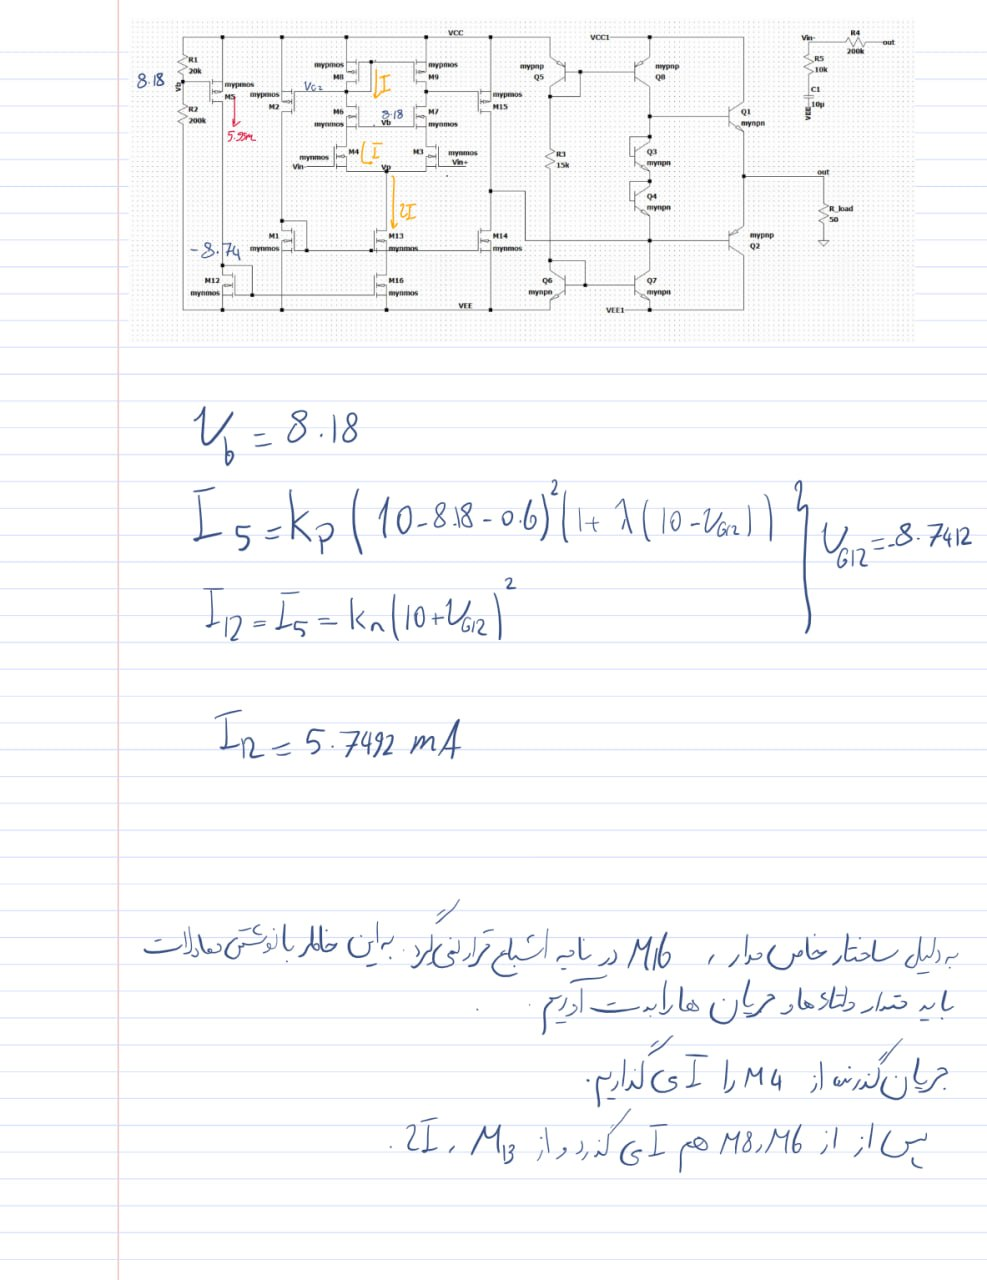
\includegraphics[width=\textwidth]{bias1.png}
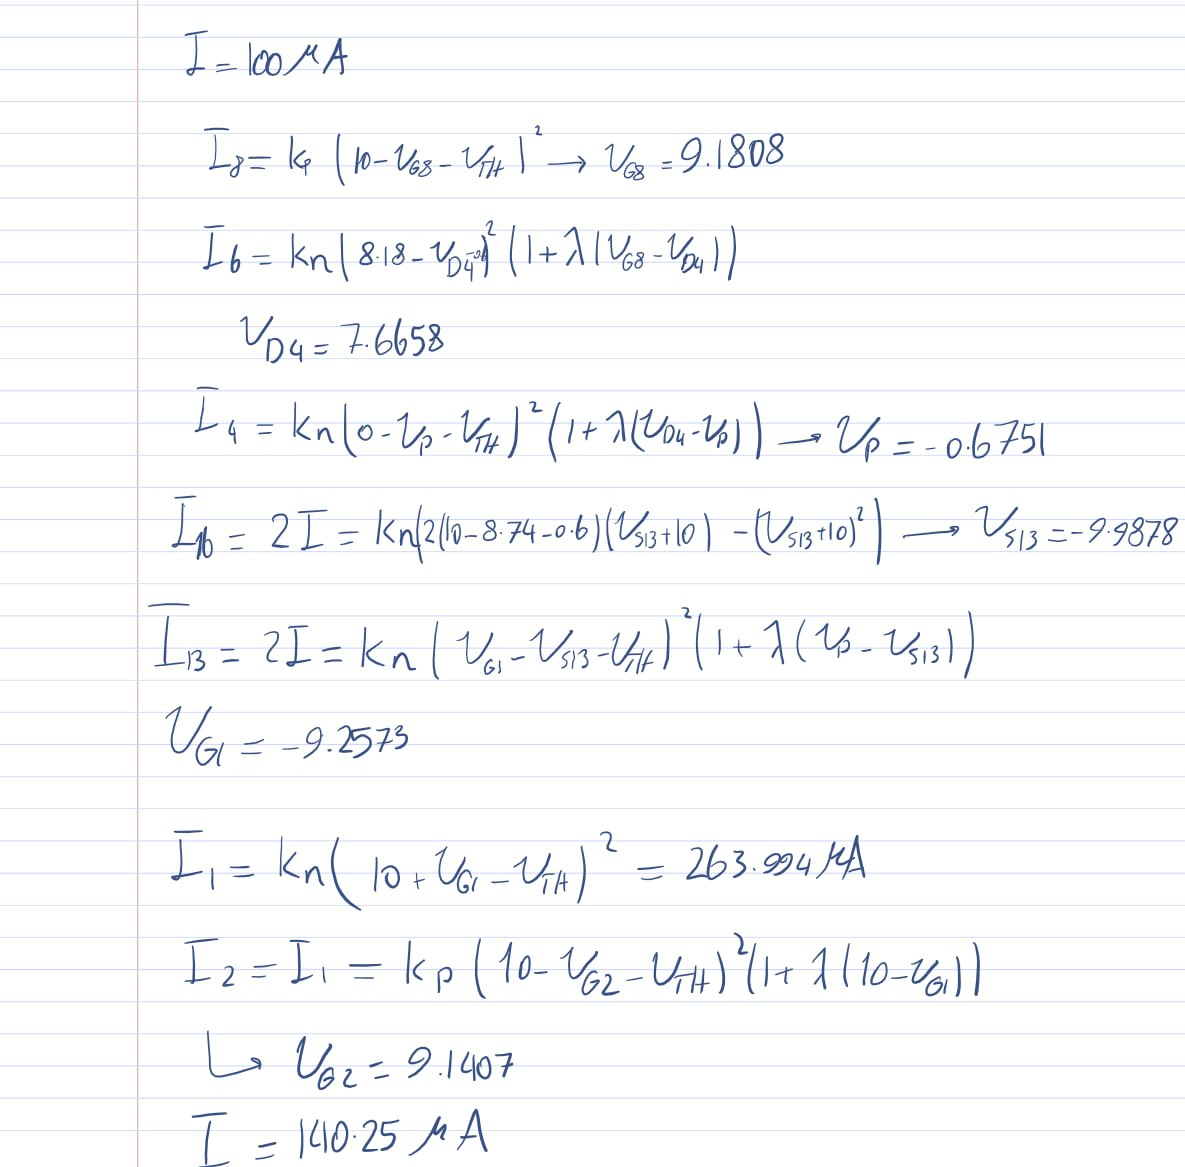
\includegraphics[width=\textwidth]{bias2.png}
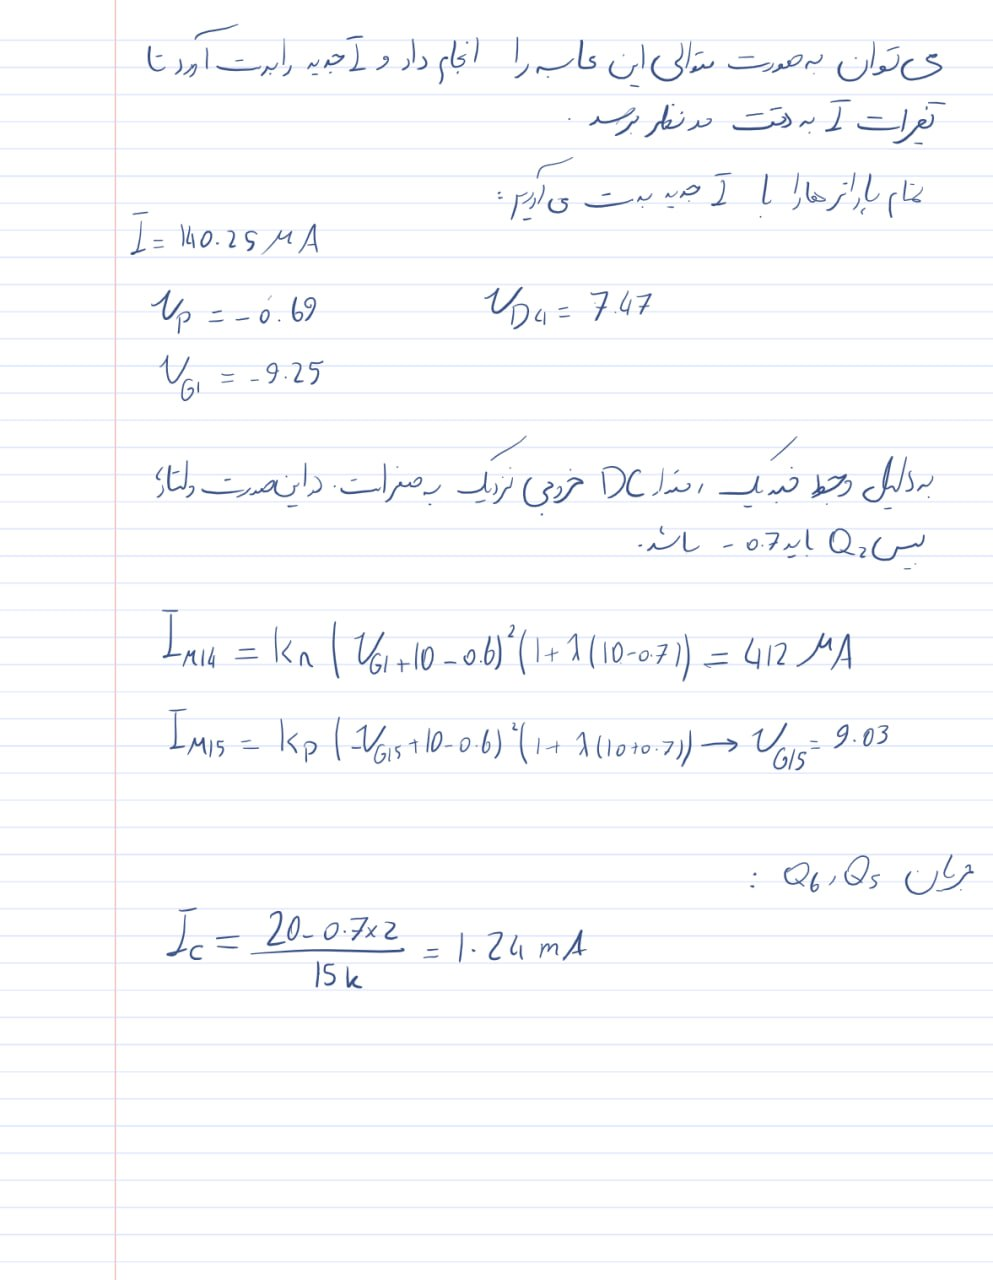
\includegraphics[width=\textwidth]{bias3.png}
\end{center}

\end{calcbox}

\begin{answerbox}{نتایج شبیه‌سازی DC Operating Point}
در این قسمت خروجی شبیه‌سازی نقطه کار DC را قرار دهید و مقادیر مهم را استخراج کنید.


\begin{center}
	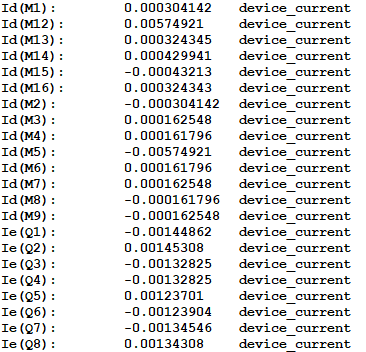
\includegraphics[width=0.8\textwidth]{bias_sim1.png}
		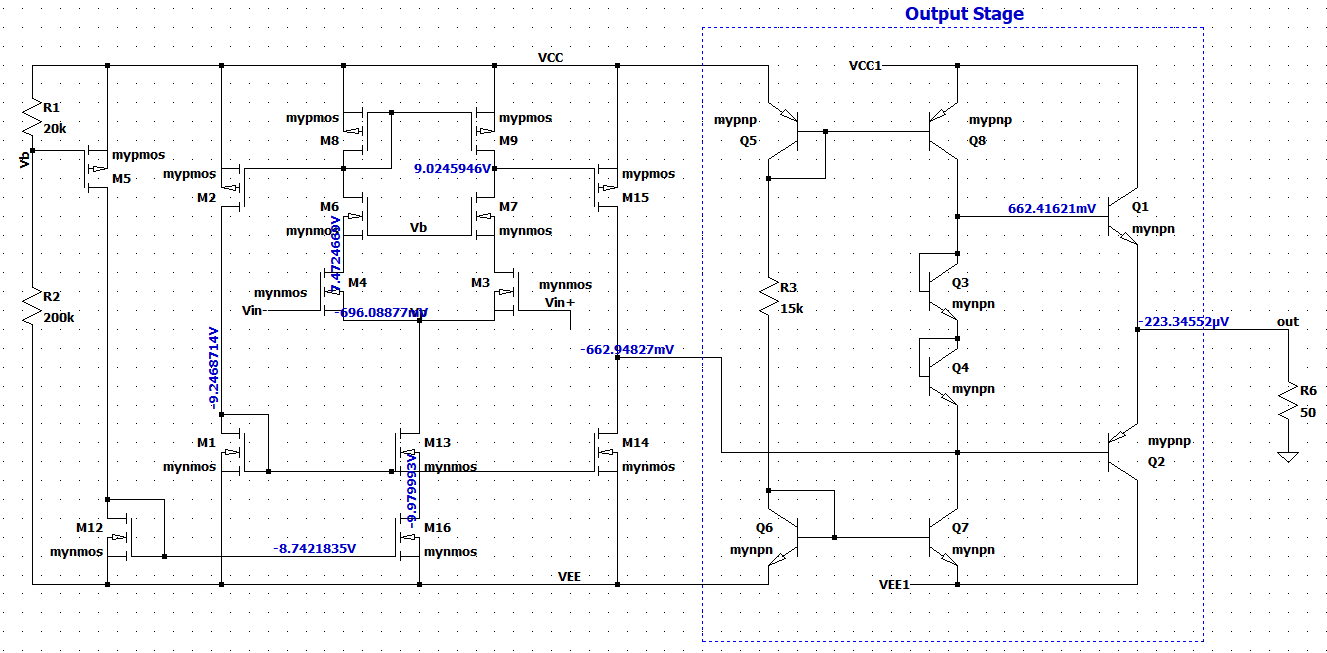
\includegraphics[width=\textwidth]{bias_sim2.png}
\end{center}

\vspace{1cm}

\textbf{نتایج مهم:}
\begin{itemize}
    \item ولتاژ DC خروجی در حالت ورودی صفر: \underline{$223\, \mu V$}
    \item جریان بایاس طبقه خروجی: \underline{$1.33\, mA$}
    \item توضیح کوتاه درباره‌ی وضعیت بایاس و پایداری آن: \underline{}
\end{itemize}
\end{answerbox}

\newpage

% =============================================================================
% SECTION 3
% =============================================================================
\section{طراحی طبقه خروجی توان}

\begin{taskbox}{خواسته مسئله (بخش ۳)}
طبقه خروجی توان را معرفی و تحلیل کنید. باید نشان دهید که این طبقه به‌صورت یکپارچه به مدار اصلی متصل شده و برای راه‌اندازی بار $50\Omega$ طراحی شده است. در این بخش نحوه اتصال، نوع ترانزیستورها، بایاس‌گذاری و دلایل انتخاب ساختار را توضیح دهید.
\end{taskbox}

\begin{calcbox}{تحلیل و محاسبات تئوری طبقه خروجی}پ
برای ولتاژ $Vpp = 16 V$ داریم:
$$I = \frac{8}{50} = 160 \, mA$$
$$P = \frac{V_p^2}{2 R_L} = 0.64 \, W$$
$$P_{supply} = \frac{2V_{CC} V_p}{\pi R_L}$$
$$\to \quad \eta = \frac\pi4 \frac{V_p}{V_{CC}}$$
در حالت ایده‌آل که بتواند $V_p = V_{CC}$ بشود، $\eta = 78.5\%$ بدست می‌آید، ولی برای $V_p = 8$‌اگر محاسبه بکنیم:
$$\eta \approx 63 \% $$

\end{calcbox}

\begin{answerbox}{معرفی و ارزیابی طبقه خروجی}
	از درین ترانزیستور 
	$M15$ 
	که خروجی طبقه تقویت ولتاژ است، به طبقه خروجی متصل می‌کنیم. ترانزیستور‌های $Q5$ و $Q6$ جریان لازم برای راه اندازی طبقه خروجی را تامین می‌کنند.
	ترانزیستور‌های $Q3$ و $Q4$ از بوجود آمدن \lr{Dead-zone} جلوگیری می‌کنند و $Q8$ و $Q7$ جریان مدار بایاس را کپی می‌کنند. ای ساختار به راحتی جریان لازم برای بار را فراهم کرده و هیچ اعوجاجی در سیگنال خروجی دیده نمی‌شود.
	\begin{center}
		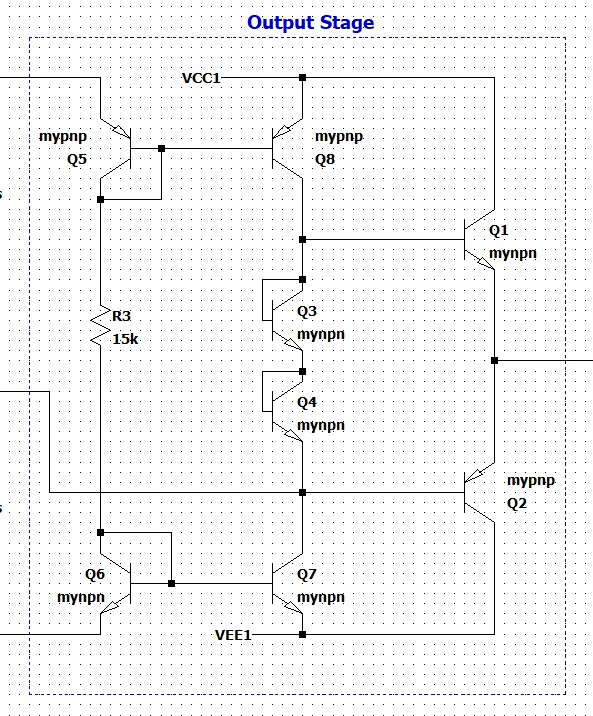
\includegraphics[width =0.7 \textwidth]{OutputStage.jpg}
	\end{center}
\end{answerbox}

\newpage

% =============================================================================
% SECTION 4
% =============================================================================
\section{اعمال فیدبک منفی سراسری}

\begin{taskbox}{خواسته مسئله (بخش ۴)}
پس از افزودن طبقه خروجی، فیدبک منفی سراسری را روی مدار کامل اعمال کنید. فیدبک باید از خروجی نهایی مدار گرفته شود و به ورودی تفاضلی بازگردد. شبکه اصلی فیدبک فقط باید شامل دو مقاومت $R_f$ و $R_g$ باشد و بهره حلقه‌بسته باید تقریباً برابر $20$ شود.
\end{taskbox}

\begin{calcbox}{محاسبات تئوری شبکه فیدبک}
	اگر بهره مدار باز این مدار برابر باشد با $a$ و بهره فیدبک $f$ باشد، بهره نهایی مدار می‌شود،
	\begin{equation}
		A = \frac{a}{1 + a\cdot f}
	\end{equation}
	اگر مقدار $a$ زیاد باشد،‌آنگاه می‌توان نوشت:
	\begin{equation}
		A = \frac{1}{f}
	\end{equation}
	حال به طراحی مدار فیدبک بپردازیم. از دو مقاومت استفاده شده است و خروجی مدار را به ورودی منفی وصل می‌کند. از خازن هم استفاده شده است که $VEE$ مشابه زمین برای AC رفتار بکند. 
مقادیر مقاومت‌ها به نوعی انتخاب شده‌اند که در نهایت $f = \frac{1}{20}$ بدهد. 
\end{calcbox}

\begin{answerbox}{نتایج اعمال فیدبک}
\textbf{مقادیر نهایی:}
\begin{itemize}
    \item $R_f$: \underline{$200 \, k \Omega$}
    \item $R_g$: \underline{$10 \, k \Omega$}
    \item محل نمونه‌برداری فیدبک: \underline{خروجی مدار که با لیبل \lr{\texttt{out}} نشان داده است.}
    \item محل اعمال فیدبک: \underline{به ترمینال منفی ورودی دیفرانسیلی.}
\end{itemize}

\vspace{1cm}

\textbf{بهره حلقه‌بسته در $1\,\text{kHz}$:}
\begin{itemize}
    \item $|A_{v,\text{closed}}|$: \underline{$20.92$}
    \item $20\log|A_{v,\text{closed}}|$: \underline{$26.41 \, dB$}
\end{itemize}

\begin{center}
	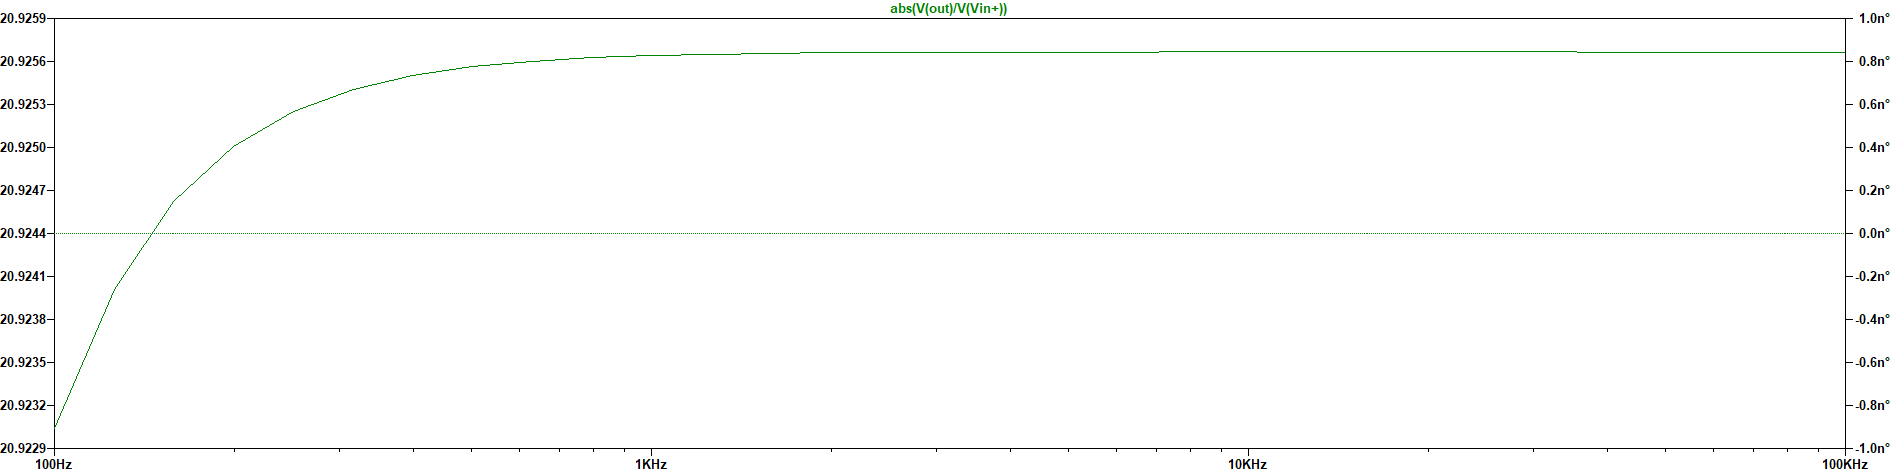
\includegraphics[width = \textwidth]{AC_simulation.png}
\end{center}



\end{answerbox}

\newpage

% =============================================================================
% SECTION 5
% =============================================================================
\section{مقایسه عملکرد مدار با فیدبک و بدون فیدبک}

\begin{taskbox}{خواسته مسئله (بخش ۵)}
مدار کامل را در دو حالت با فیدبک و بدون فیدبک مقایسه کنید. در هر دو حالت طبقه خروجی باید در مدار باقی بماند. اگر در حالت بدون فیدبک مدار اشباع می‌شود، اثر این موضوع را بر تخمین بهره توضیح دهید.
\end{taskbox}

\begin{answerbox}{مقایسه کیفی و کمی دو حالت}
به دلیل اینکه در حالت باز،‌ ضریب تقویت ولتاژ بالایی دارد با ولتاژ‌های پایین ورودی دچار \lr{clipping} می‌شویم. با تحلیل فرکانسی مدار متوجه می‌شویم که THD حدودا 10 برابری نسبت به مدار با فیدبک دارد، نشان می‌دهد که فیدبک به شدت اعوجاجات خروجی را کاهش می‌دهد و مدار را به حالت خطی نزدیک تر ‌می‌کند. تحلیل AC مدار در شکل زیر نشان داده شده است و همانطور که می‌بینید با اینکه در بازه نسبتا بزرگی بهره ثابت می‌دهد ولی این ناحیه کوچکتر از با حالت فیدبک دار است. 
\begin{center}
	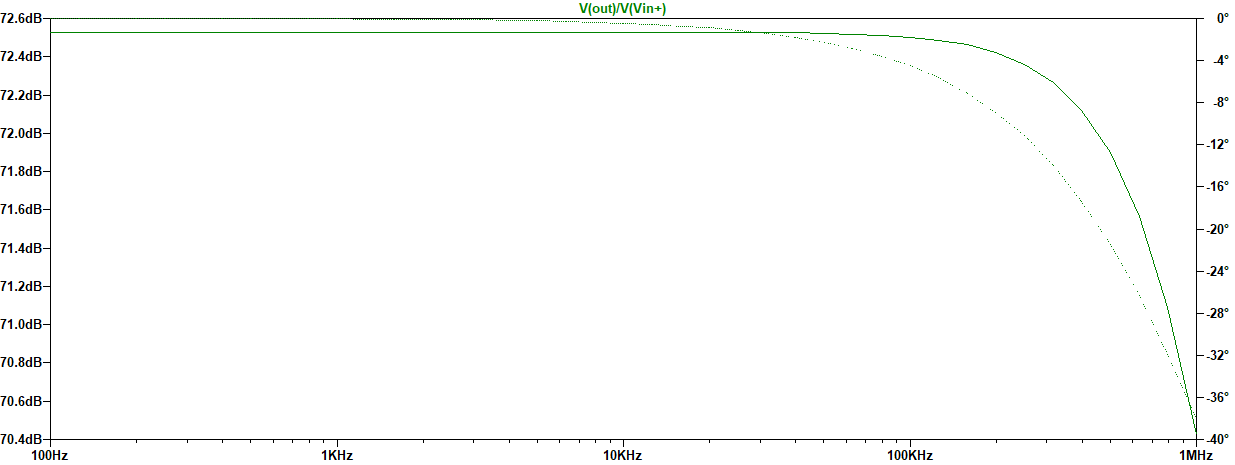
\includegraphics[width=0.8\linewidth]{AC_sim_open}
\end{center}
\end{answerbox}

\newpage
% =============================================================================
% SECTION 6
% =============================================================================
\section{تحلیل سویینگ خروجی، توان و راندمان}

\begin{taskbox}{خواسته مسئله (بخش ۶)}
بررسی کنید آیا مدار نهایی می‌تواند روی بار $50\Omega$ خروجی سینوسی با دامنه $16V_{pp}$ بدون \lr{clipping} شدید و اعوجاج آشکار ایجاد کند یا خیر. سپس توان تحویلی به بار، توان مصرفی کل مدار و راندمان طبقه خروجی را اندازه‌گیری کنید.
\end{taskbox}

\begin{calcbox}{محاسبات تئوری سویینگ و راندمان}
حداکثر سویینگ با فرض آنکه جریان کافی طبقه خروجی می‌تواند تولید بکند، 9 تا منفی 9 است.

$$P_L = \frac{V_p^2}{2 R_L} = 0.64 \, W$$

\end{calcbox}

\begin{answerbox}{نتایج شبیه‌سازی Transient و اندازه‌گیری توان}
\begin{center}
	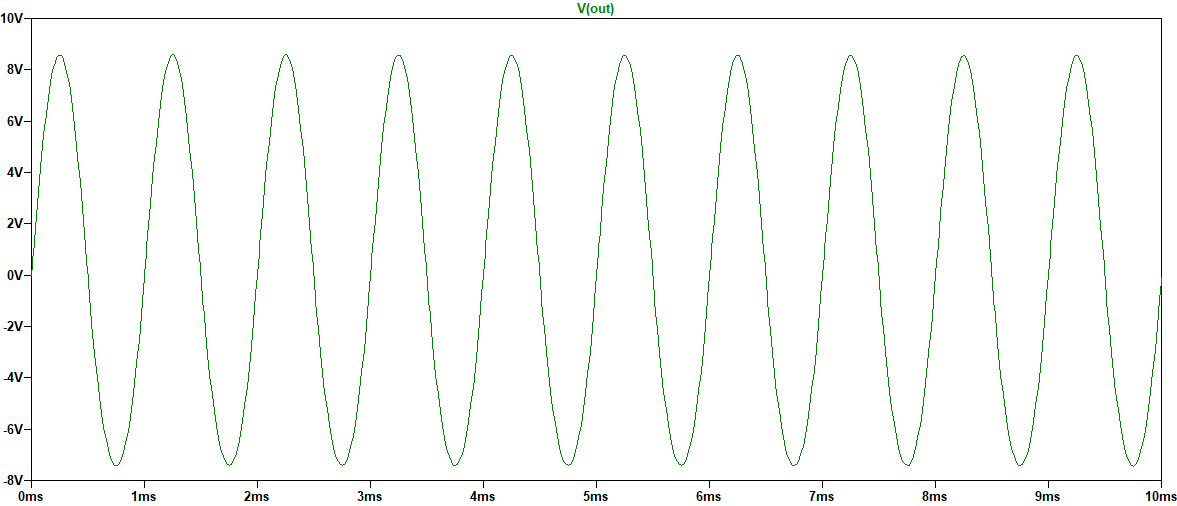
\includegraphics[width=0.8\linewidth]{max_swing.png}
		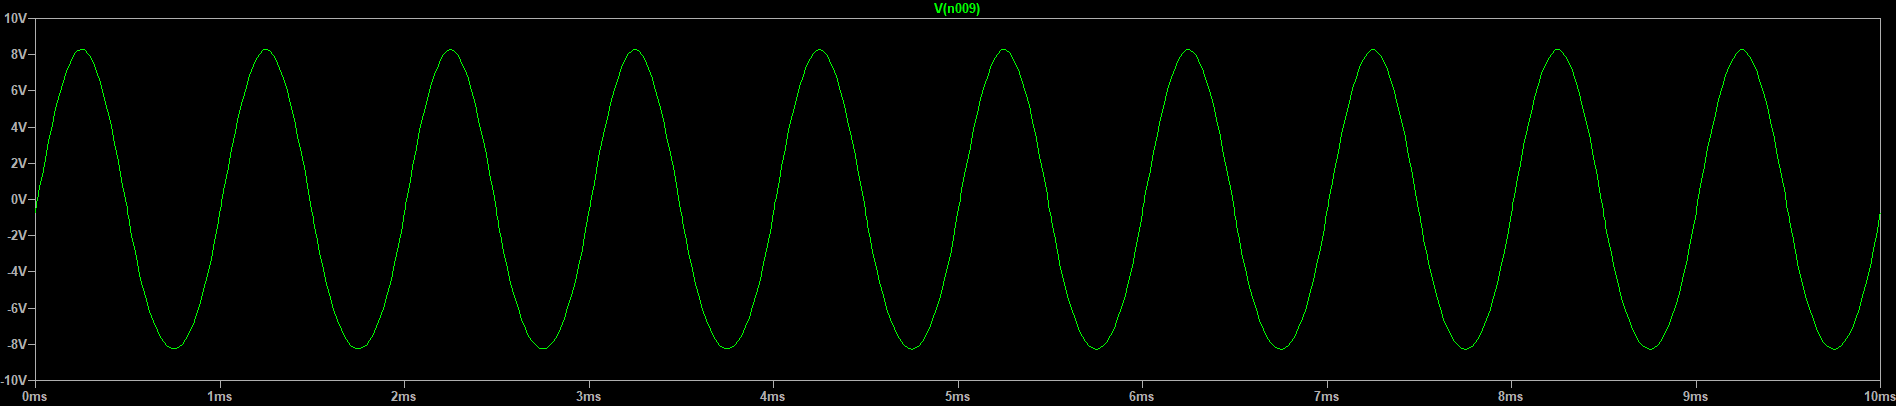
\includegraphics[width=0.8\linewidth]{max_swing2.png}
\end{center}


\textbf{نتایج عددی:}
\begin{itemize}
    \item دامنه ورودی موردنیاز برای $16V_{pp}$: \underline{$412 \, mV$}
    \item $P_{R_L}$: \underline{$804 \, mW$}
    \item $P_{\text{total}}$: \underline{$1.342 \, W$}
    \item $P_{\text{out-stage}}$: \underline{$1.163 \, W$}
    \item $\eta_{\text{out}}$: \underline{$69 \%$}
\end{itemize}
    $$
    \eta_{\text{out}}=\frac{P_{R_L}}{P_{\text{out-stage}}}\times 100\%
    $$

\vspace{1cm}

\textbf{دستورات مورد استفاده در شبیه‌سازی:}
\begin{latin}
\begin{lstlisting}[language={}]
.meas TRAN P_R_l RMS V(out)*I(R_load)
.meas TRAN P RMS V(Vcc)*I(vcc)-V(Vee)*I(vee)
\end{lstlisting}
\end{latin}
\end{answerbox}

\newpage

% =============================================================================
% SECTION 7
% =============================================================================
\section{توان مصرفی در ورودی مشخص}

\begin{taskbox}{خواسته مسئله (بخش ۷)}
برای ورودی سینوسی با دامنه $50mV$ و فرکانس $1\,\text{kHz}$، توان مصرفی کل مدار نهایی را اندازه‌گیری کنید و با شرط
$$P_{\text{total}} \le 190mW$$
مقایسه نمایید.
\end{taskbox}

\begin{answerbox}{اندازه‌گیری توان مصرفی در شرط استاندارد}
در این قسمت نتیجه‌ی اندازه‌گیری توان کل مدار در شرایط استاندارد پروژه را گزارش کنید.

\begin{center}
\begin{tabular}{|c|c|}
\hline
\textbf{پارامتر} & \textbf{مقدار} \\
\hline
دامنه ورودی & $50mV$ \\
\hline
فرکانس ورودی & $1\,\text{kHz}$ \\
\hline
توان مصرفی کل مدار & $337 \, mW$\\
\hline
وضعیت قبولی &بیشتر از مقدار قبولی است. \\
\hline
\end{tabular}
\end{center}

\vspace{5cm}
\end{answerbox}

\newpage

% =============================================================================
% SECTION 8
% =============================================================================
\section{اندازه‌گیری اعوجاج هارمونیکی کل \lr{THD}}

\begin{taskbox}{خواسته مسئله (بخش ۸)}
مقدار $THD$ را برای مدار نهایی فیدبک‌دار، با حضور طبقه خروجی و بار $50\Omega$ اندازه‌گیری کنید. آزمون باید برای ورودی سینوسی با دامنه $50mV$ و فرکانس $1\,\text{kHz}$ انجام شود. سپس همین آزمون را در حضور منبع نویزی سری‌شده با مقاومت‌های تعیین‌کننده جریان منابع جریان تکرار کنید.
\end{taskbox}

\begin{calcbox}{روش اندازه‌گیری و تحلیل نتایج}
منبع نویز را سری شده است با مقاومت‌های $R2$ و $R3$. همچنان به نظر تاثیری زیادی بر THD نگذاشتند.


بدون نویز: $THD = 0.064$

با وجود منابع نویز: $THD = 0.065$

\textbf{دستور پیشنهادی:}
\begin{latin}
\begin{lstlisting}[language={}]
.FOUR 1khz 100 V(out)
\end{lstlisting}
\end{latin}

\vspace{4cm}
\end{calcbox}

\begin{answerbox}{نتایج آزمون $THD$}
\begin{center}
\begin{tabular}{|c|c|c|}
\hline
\textbf{شرایط آزمون} & \textbf{مقدار $THD$} & \textbf{وضعیت} \\
\hline
مدار فیدبک‌دار، بدون منبع نویزی & $0.064$ & باید کمتر از $0.08\%$ باشد \\
\hline
مدار فیدبک‌دار، با منبع نویزی سری‌شده & $0.065$& باید کمتر از $1\%$ باشد \\
\hline
\end{tabular}
\end{center}


\vspace{1cm}

\textbf{توضیح کوتاه درباره تغییر $THD$ در حضور نویز:}

\vspace{4cm}
\end{answerbox}

\newpage

% =============================================================================
% SECTION 9
% =============================================================================
\section{اندازه‌گیری \lr{PSRR} با منبع تغذیه دندانه‌اره‌ای}

\begin{taskbox}{خواسته مسئله (بخش ۹)}
با صفر کردن ورودی مدار، اثر ریپل منبع تغذیه را بر خروجی بررسی کنید. در این آزمون باید از منابع تغذیه دندانه‌اره‌ای با ریپل $10mV$ برای $V_{CC}$ و $V_{EE}$ استفاده شود و سپس مقدار $PSRR$ از رابطه
$$
PSRR = 20\log\left(\frac{V_{\text{ripple}}}{\Delta V_{out}}\right)
$$
محاسبه شود.
\end{taskbox}

\begin{calcbox}{روش آزمون و محاسبه $PSRR$}
	$$PSRR = -25\, dB$$
\textbf{نمونه منبع پیشنهادی:}
\begin{latin}
\begin{lstlisting}[language={}]
Vcc Vcc 0 PWL(0 12 5m 12.01 10m 12 15m 12.01 20m 12)
Vee Vee 0 PWL(0 -12 5m -12.01 10m -12 15m -12.01 20m -12)
\end{lstlisting}
\end{latin}

\vspace{3cm}
\end{calcbox}

\begin{answerbox}{نتایج آزمون $PSRR$}
\begin{center}
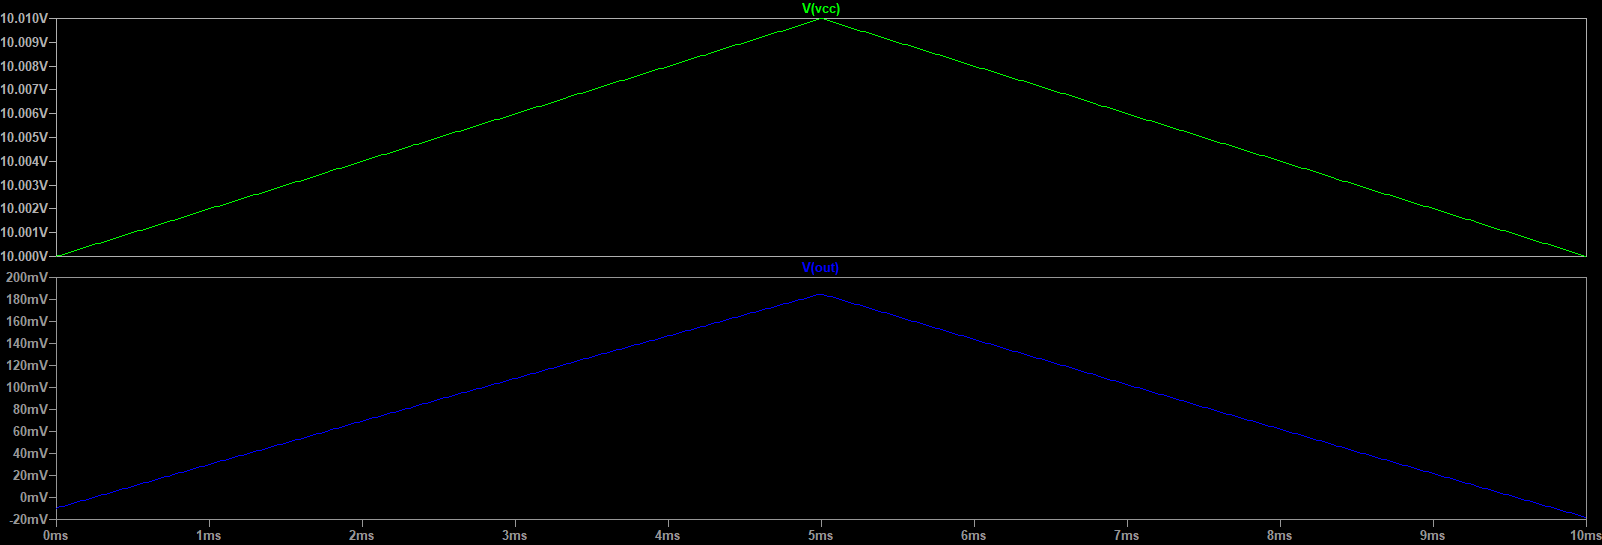
\includegraphics[width=0.85\textwidth]{PSRR.png}
\end{center}
\vspace{3cm}

\begin{center}
\begin{tabular}{|c|c|}
\hline
\textbf{پارامتر} & \textbf{مقدار} \\
\hline
$V_{\text{ripple}}$ &$10 mV$ \\
\hline
$\Delta V_{out}$ & $180 \, mV$\\
\hline
$PSRR$ & $ -25\, dB$\\
\hline
\end{tabular}
\end{center}

\vspace{1cm}

\textbf{توضیح کوتاه درباره عملکرد مدار در برابر ریپل منبع تغذیه:}

\vspace{4cm}
\end{answerbox}

\newpage

% =============================================================================
% SECTION 10
% =============================================================================
\section{اندازه‌گیری مقاومت ورودی تفاضلی}

\begin{taskbox}{خواسته مسئله (بخش ۱۰)}
مقاومت ورودی تفاضلی مدار نهایی را اندازه‌گیری کنید و با شرط
$$R_{in,\text{diff}} > 1M\Omega$$
مقایسه نمایید. روش اندازه‌گیری باید به‌طور کامل توضیح داده شود.
\end{taskbox}

\begin{calcbox}{محاسبات یا روش تحلیلی مقاومت ورودی تفاضلی}
به دلیل آنکه از ترانزیستور‌های ماسفت استفاده شده است، مقاومت ورودی بی‌نهایت داریم.
\vspace{1cm}
\end{calcbox}

\newpage

% =============================================================================
% SECTION 11
% =============================================================================
\section{اندازه‌گیری مقاومت خروجی}

\begin{taskbox}{خواسته مسئله (بخش ۱۱)}
مقاومت خروجی مدار نهایی را پس از حذف بار $R_L$ اندازه‌گیری کنید و با شرط
$$R_{out} < 50\Omega$$
مقایسه نمایید. روش شبیه‌سازی و استخراج مقدار باید توضیح داده شود.
\end{taskbox}

\begin{calcbox}{محاسبات یا روش تحلیلی مقاومت خروجی}
در این بخش روش تئوری یا تخمین تحلیلی مقاومت خروجی را بنویسید.

\begin{center}
\textcolor{gray}{\small{محاسبات مربوط به $R_{out}$ را اینجا قرار دهید}}

% \includegraphics[width=0.95\textwidth]{rout_phase2_calc.jpg}
\end{center}
\vspace{5cm}
\end{calcbox}

\begin{answerbox}{نتایج شبیه‌سازی مقاومت خروجی}
در حالت بی‌باری اول ولتاژ اندازه‌گیری می‌شود. سپس یک مقاومت تست به خروجی اضافه می‌کنیم. با تغییر دادن می‌توانیم مقدار دامنه ولتاژ خروجی را کاهش بدهیم. زمانی که این مقدار به نصف مقدار حالت بی‌باری برسد،‌آن مقاومت با مقاومت خروجی مدار برابر است.


\begin{center}
	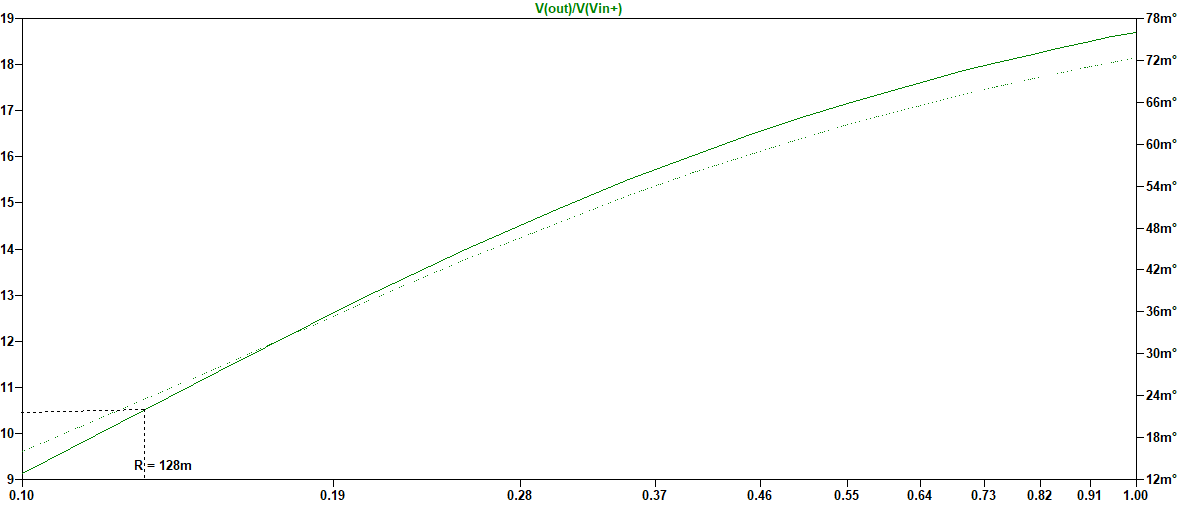
\includegraphics[width=0.7\linewidth]{Rout_sim}
\end{center}

\textbf{مقدار نهایی:}
\begin{itemize}
    \item $R_{out}$: \underline{$R_{out} = 128 \, m \Omega$}
    \item وضعیت قبولی: \underline{در شرط گفته شده صدق می‌کند.}
\end{itemize}
\end{answerbox}

\newpage

% =============================================================================
% SECTION 12
% =============================================================================
\section{آزمون تقویت سیگنال صوتی واقعی}

\begin{taskbox}{خواسته مسئله (بخش ۱۲)}
در این بخش باید یک فایل صوتی واقعی به ورودی مدار اعمال شود و خروجی تقویت‌شده بررسی گردد. استفاده از سیگنال سینوسی ساده به‌جای فایل صوتی واقعی قابل قبول نیست. لازم است شکل موج ورودی و خروجی قرار داده شود و نشان داده شود که خروجی دچار \lr{clipping} شدید نشده است.
\end{taskbox}

\begin{calcbox}{آماده‌سازی فایل صوتی و توضیحات لازم}
در این بخش مشخص کنید:
\begin{itemize}
    \item فایل ورودی از چه نوعی بوده است
    \item آیا به تک‌کاناله تبدیل شده است یا خیر
    \item نرخ نمونه‌برداری چقدر بوده است
    \item آیا دامنه نرمال‌سازی شده است یا خیر
\end{itemize}


\vspace{2cm}
\end{calcbox}

\begin{answerbox}{نتایج آزمون صوتی}
\textbf{مشخصات فایل صوتی:}
\begin{itemize}
    \item نام فایل ورودی: \underline{\texttt{input.wav}}
    \item نام فایل خروجی: \underline{\texttt{output.wav}}
    \item \lr{fft} فایل ورودی و خروجی

\end{itemize}

\begin{center}
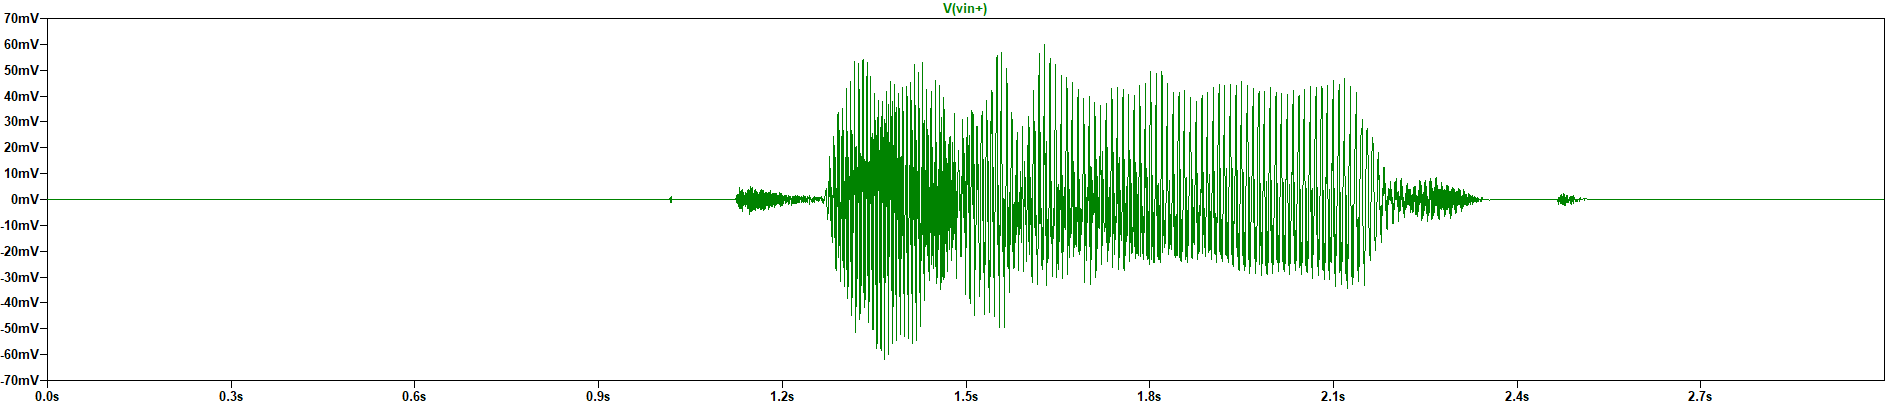
\includegraphics[width=0.85\textwidth]{audio_input_waveform.png}
\end{center}
\vspace{2cm}

\begin{center}
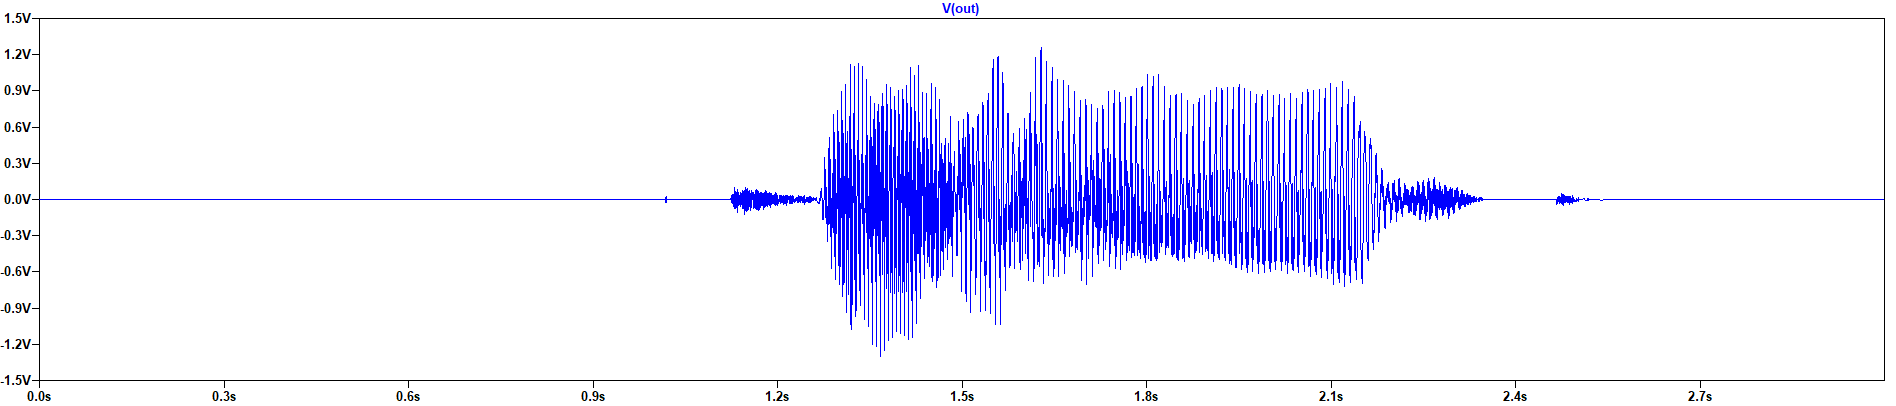
\includegraphics[width=0.85\textwidth]{audio_output_waveform.png}
\end{center}
\vspace{2cm}

\begin{center}
	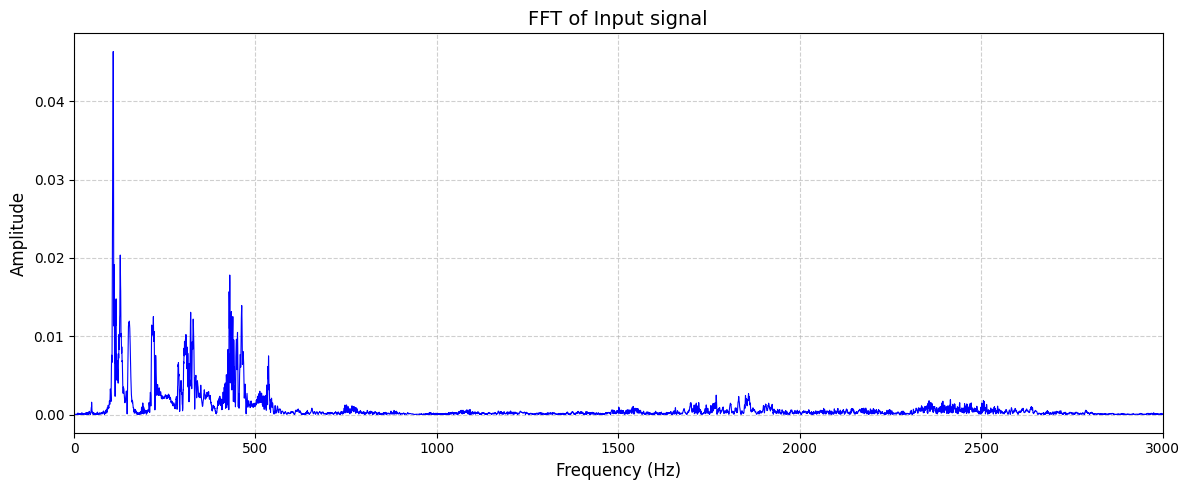
\includegraphics[width=0.85\textwidth]{FFT_input.png}
\end{center}
\vspace{2cm}

\begin{center}
	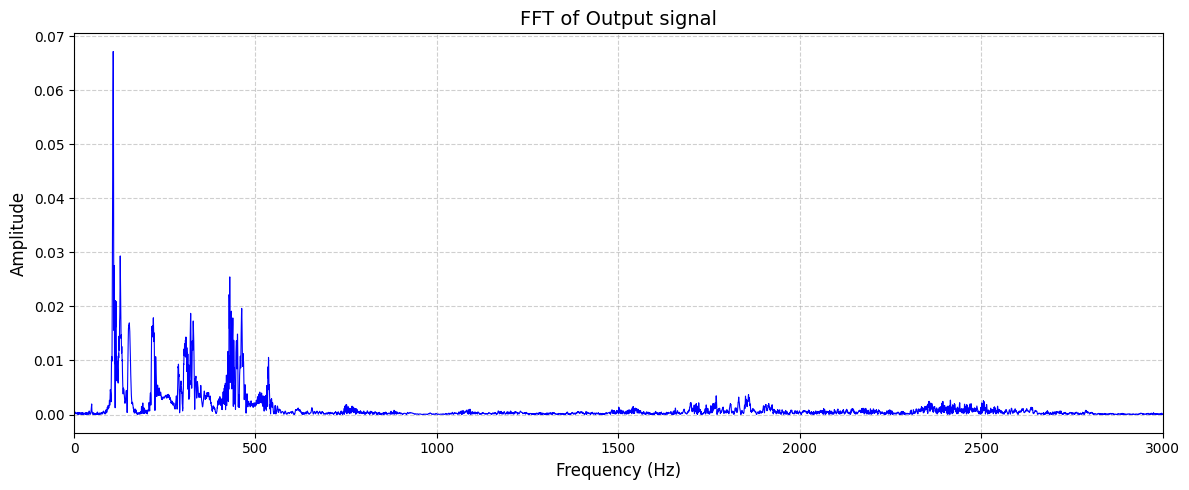
\includegraphics[width=0.85\textwidth]{FFT_output.png}
\end{center}
\vspace{2cm}
\textbf{توضیح درباره کیفیت خروجی و وجود یا عدم وجود \lr{clipping}:}

فایل خروجی بدون هیج اعوجاج مشهودی ایجاد شده است. با فقط گوش دادن به آن متوجه‌ی هیچ اعوجاجی نمی‌شویم و فقط سیگنال ورودی را به صورت تقویت شده داریم. 

\end{answerbox}

\newpage

% =============================================================================
% SECTION 13
% =============================================================================
\section{هزینه مدار و محدودیت قطعات}

\begin{taskbox}{خواسته مسئله (بخش ۱۳)}
هزینه نهایی مدار خود را با توجه به فایل محاسبه هزینه تعیین کنید. اگر هزینه از $200$ بیشتر شده است، مقدار جریمه را از رابطه زیر محاسبه کنید:
$$
\text{Penalty} = 2\% \times \left\lceil \frac{\text{Cost}-200}{5} \right\rceil
$$
\end{taskbox}

\begin{answerbox}{جدول تعداد قطعات و هزینه}
\begin{center}
\begin{tabular}{|c|c|c|c|}
\hline
\textbf{نوع المان} & \textbf{تعداد} & \textbf{هزینه هر واحد} & \textbf{هزینه کل} \\
\hline
MOSFET & $14$ & $3$ & $42$ \\
\hline
BJT & $8$ & $5$ & $40$ \\
\hline
مقاومت & $5$ & $10$ &$50$ \\
\hline
خازن & $1$ & $40$ &$40$\\
\hline
\multicolumn{3}{|c|}{\textbf{هزینه کل}} &$172$ \\
\hline
\end{tabular}
\end{center}

\vspace{1cm}

\textbf{نتایج:}
\begin{itemize}
    \item هزینه کل مدار: \underline{$172$}
    \item آیا از سقف هزینه عبور کرده‌اید؟ \underline{خیر}
\end{itemize}

\vspace{4cm}
\end{answerbox}

\newpage

% =============================================================================
% SECTION 14
% =============================================================================
\section{شرایط امتیازی پروژه}

\begin{taskbox}{خواسته مسئله (بخش ۱۴)}
اگر شرایط امتیازی پروژه را بررسی کرده‌اید، در این بخش نتایج آن را گزارش کنید. برای دریافت امتیاز اضافه باید هر سه شرط زیر هم‌زمان برقرار باشند:
\begin{itemize}
    \item سویینگ خروجی $17V_{pp}$ بدون \lr{clipping} آشکار
    \item راندمان بیشتر از $70\%$ در همان نقطه کاری
    \item ولتاژ DC خروجی کمتر از $100mV$
\end{itemize}
\end{taskbox}

\begin{answerbox}{بررسی شرایط امتیازی}
	در این مدار گزارش شده تا اینجای کار، نمی‌توان شرایط امتیازی را برآورده کرد. ولی با یک تغییر کوچک در مقدار مقاومت $R_3$ امکان پذیر است. اگر $R_3$ را از $17k$ به $12k$ کاهش بدهیم با مقدار ورودی ولتاژ $450 \, mV$ به سویینگ خواسته شده می‌رسید و راندمان در این شرایط $74\%$ است و همینطور حد ولتاژ DC خواسته شده را هم دارا است. 
	
	با تغییر مقدار $R_3$ تغییر زیادی در پارامتر‌های حساب شده تا اینجای کار بوجود نمی‌آید، فقط توان مصرفی کل افزایش میابد که در مدار قبلی هم از $190 \, mW$ بیشتر است. به همین خاطر تمام خواسته‌هایی که مدار قبلی برآورده می‌کند با تغییر مقاومت هم خواهیم داشت. 
\begin{center}
\begin{tabular}{|c|c|c|}
\hline
\textbf{پارامتر} & \textbf{شرط لازم} & \textbf{مقدار شما} \\
\hline
سویینگ خروجی & $17V_{pp}$ & \\
\hline
راندمان & $>70\%$ & \\
\hline
$|V_{out,DC}|$ & $<100mV$ & \\
\hline
\end{tabular}
\end{center}

\vspace{1cm}

\textbf{موارد لازم:}
\begin{itemize}
    \item دامنه ورودی متناظر با $17V_{pp}$: \underline{\hspace{4cm}}
    \item شکل موج خروجی در این حالت: \underline{\hspace{4cm}}
    \item نتیجه نهایی بخش امتیازی: \underline{\hspace{4cm}}
\end{itemize}

\vspace{5cm}
\end{answerbox}

\newpage

% =============================================================================
% SECTION 15
% =============================================================================
\section{فایل‌های تحویلی}

\begin{taskbox}{خواسته مسئله (بخش ۱۵)}
فهرست فایل‌های نهایی تحویلی پروژه را کامل کنید.
\end{taskbox}

\begin{answerbox}{چک‌لیست فایل‌های تحویلی}
\begin{itemize}
    \item فایل شماتیک مدار کامل \lr{LTspice} با پسوند \lr{.asc}
    \item فایل مربوط به آزمون صوتی
    \item فایل \lr{audio.wav}
    \item فایل \lr{output.wav}
    \item گزارش نهایی به‌صورت \lr{PDF}
\end{itemize}

\vspace{5cm}
\end{answerbox}

\newpage

% =============================================================================
% SECTION 16
% =============================================================================
\section{جمع‌بندی نهایی}

\begin{taskbox}{خواسته مسئله (بخش ۱۶)}
در یک جمع‌بندی کوتاه توضیح دهید:
\begin{itemize}
    \item مهم‌ترین چالش طراحی فاز دوم چه بود؟
    \item کدام بخش از میان طبقه خروجی، فیدبک، $THD$، $PSRR$ یا تست صوتی سخت‌تر بود؟
    \item اگر بعضی مشخصات به‌طور کامل برآورده نشده‌اند، علت آن چیست؟
    \item اگر زمان یا هزینه بیشتری داشتید چه بهبودی در مدار اعمال می‌کردید؟
\end{itemize}
\end{taskbox}

\begin{answerbox}{نتیجه‌گیری نهایی}
در اول سعی داشتم که با استفاده از مدار فاز قبلی و با بهبود آن مدار این فاز را طراحی بکنم. به دلیل محدودیت هزینه و توان مصرفی موفق به این کار نشدم. با طراحی دوباره با ماسفت توانستم هزینه را کاهش بدهم ولی همچنان توان مصرفی بالاتر از حد مجاز است. با این حال به نظر طراحی جدید این فاز بهتر از فاز قبل توانست شرایط این فاز را برقرار بکند.

اگر زمان  بیشتری برای طراحی داشتم احتمالا به دنبال راهی برای کاهش دادن توان مصرفی می‌گشتم. ولی به غیر از آن عملکرد مدار در بقیه بخش‌ها قابل قبول است. 


\end{answerbox}

\end{document}
